\documentclass[11pt]{article}
\usepackage{mathtools}
\usepackage{mdframed}
\usepackage{fullpage}
\usepackage{amsfonts}
\usepackage{tikz}
\usepackage{hyperref}
\usepackage{pdfpages}



%edit this for each class
\newcommand\name{John Vincent}
\newcommand\classname{}
\newcommand\assignment{}



\newcounter{excounter}
\setcounter{excounter}{1}
\newcommand\question[2]{\vskip 1em  \noindent\textbf{\arabic{excounter}\addtocounter{excounter}{1}.} \emph{#1} \noindent#2}


% You can also erase this if you do not have package fancyhdr
% Fancy footnote.........
\usepackage{fancyhdr}  %% If it does not work with your latex installation, you may just delete this...
\pagestyle{fancy}
\usepackage{lastpage}
\rfoot{\name, page \thepage/\pageref{LastPage}}
\cfoot{}
\rhead{}
\lhead{}
\renewcommand{\headrulewidth}{0pt}
\renewcommand{\footrulewidth}{0pt}
\DeclarePairedDelimiter\ceil{\lceil}{\rceil}
\DeclarePairedDelimiter\floor{\lfloor}{\rfloor}



\begin{document}


  \hfill \name\\
  \null\hfill Topic Proposal\\
  \vskip 1em

  \noindent\large{\textbf{Problem Statement}}

  \noindent On August 25, 1991 a man named Linus Torvalds posted a message announcing his new creation. It was a free kernel that was developed to mimic the behavior of the very popular UNIX terminal.
  Since he released the source code for others to use, they were able to help build features into this new creation(Hayward 2012, p.1). In only a few years different branches of development centered around this
  kernel started to sprout up, and iterations continue to be developed to this day, the most famous being the Android platform which runs 38\% of computers in the world(Operating System Market 2017).\\

  \noindent Due to the open nature of development this operating system is easy for knowledgeable people to take apart and rebuild to better fit the needs of a user.
  This flexibility, efficiency, and lack of licensing fees has caused rapid adoption among companies, and developers. Servers that run Linux are on the rise at the expense of UNIX, Windows, and mainframe
  technologies, and companies have an increasing need for developers train the using Linux (Vaughan-Nichols 2015). Aside from being a marketable skill the Linux environment has many tools made for free
  by developers for developers that increase productivity, and reduce frustration. This would explain why Linux is the second most used platform and the most loved platform among professional
  developers(Stack Overflow Developer Survey 2017).\\

  \noindent Despite all these reasons to incentivise students to learn Linux there are still very few times Linux is even mentioned to Software
  Engineering students at Iowa State. The first class on the flow chart that recommends Linux is Com S 327, and it isn't even a required course since embeded systems is an alternative.
  This class also comes later in the program after most students have already become attached to a development environment, causing a reluctance to adopt a new system. This course
  also recommends a VM approach which will ultimately end up in most students only learning the bare minimum of Linux and then tossing it to the side when the course is over since they
  never actuall have the operating system installed. On top of that even if they did like using Linux the course offers no resources on how to actually install it to their system
  if they did want to make the change. So this course does give students a reason to try using Linux, but it leaves them to their own devices to learn how to set up, and
  maintain a linux installation.\\

  \noindent There is a course offered by Iowa State, Com S 252, about "Introduction to installation, utilization, and administration of Linux systems". Which would be the perfect course
  for students to learn about Linux. This course, however, isn't on the radar for most students in Software Engineering. The marketability of understanding Linux, and the productivity benefits in using Linux for development
  make this course a must for future students. This course should be added to the Software Engineering graduation requirements which will ensure that graduates from Iowa State will be able to function
  in a work environment that uses linux servers, or develops for android, which is an inevitability for a career developer.

  \noindent\large{\textbf{Solution}}

  \noindent There are a number of ways to increase Linux literacy among Iowa State's Software Engineering students. I recommend two minor changes that
  together should help the students become comfortable operating a Linux based system. These changes center around increasing the visibility of current resources
  as well as adding some more resources for areas that are currently lacking in the curriculum.\\

  \noindent The first change I am going to recommend is that Com S 252 is made into a required course. This will guarantee that all students at least have a basic knowledge of Linux, ensuring our graduates feel prepared when they encounter Linux in the field. Com S 252 can fit into the flowchart where ENGL 250 is now, and ENGL 250 can move into second semester sophomore year without interrupting the rest of the flowchart. Then either a tech elective can be removed from the senior year to make the credit requirement the same or the requirement could be increased. If the credit load per semester is a concern the GEN ED elective could be moved down into the senior year and replace and tech elective. Overall this change could be implemented with minimal changes to the flowchart, It ultimately could be viewed as forcing a specific class to be selected in place of a current elective. While this will reduce the student's control over their own education,
  the change will ultimately serve most students better, as developers that know linux are increasingly getting paid more than developers that don't(It's a Great
  Time to Know Linux).\\

  \noindent The second change I recommend is adding a system administration class. currently there are no classes that teach how to properly configure and maintain
  environments. This class would cover current server, and database applications, as well as how to configure them to run securely on a real system. Since
  Linux is the most common server technology currently this course would require students to use Linux through putty or ssh to set up a school owned server.
  This course would be offered as an elective, and would allow students that intend to work for small companies or startups to learn the essential skills
  to bring a product they design into a production environment without the need for a whole system administration department. This course would also benefit
  students working at larger companies because they would develop a deeper understanding of how their environments work, and how they can optimize/utilize the
  capabilities of their environments.\\

  \noindent{\textbf{Financial Cost}}\\
  \noindent The largest cost for implementing this plan would be adding the new class. For this class the University would need to provide a Professor, as well as
  multiple TAs to help students during office hours, as this class would be very hands on. The University would also need to set aside server space for the class,
  this is already done for multiple classes so it should be a know quantity.\\

  \clearpage

  \noindent{\textbf{Time Cost}}\\
  This plan would require the time of the administration to make the revisions to the current flowchart. Software Engineering Advisors would also
  have to manage students with different graduation requirements for a time after the change which may require some extra oversight for a period of time.
  The administration would also have to put in the time to approve the new class and find a Professor and TAs for the class. The Professor selected for the class
  would also have to spend a substantial amount of time developing, and administering the class. The IT department would have to spend time setting up the servers
  for the new class, as well as monitoring them for security purposes once they are being used. The IT department would also have to spend time resetting the
  servers after each semester to prepare for the new students coming in.\\

  \noindent\large{\textbf{Summary}}

  \noindent Currently students are not learning much about Linux systems, even though it is a high desired skill set. There are a few changes Iowa State could
  make to increase Linux literacy among its graduates to better prepare them for work in the real world. One solution is very simple with the only cost being
  limiting student choice. The other choice is quite a bit more costly, and would require more effort by the administration, but would fill a void in the current
  curriculum.

  \clearpage

  \begin{center} \large{\textbf{References}} \end{center}

  \noindent Vaughan-Nichols, Steven J. ``Linux Foundation Finds Enterprise Linux Growing at Windows'
  Expense." ZDNet, ZDNet, 4 Dec. 2015,
  www.zdnet.com/article/Linux-foundation-finds-enterprise-Linux-growing-at-windows-expense/.\\

  \noindent ``Stack Overflow Developer Survey 2017." Stack Overflow,\\ insights.stackoverflow.com/survey/2017\#most-popular-technologies.\\

  \noindent ``The Complete Beginner's Guide to Linux." Linux.com | The Source for Linux Information, 13 Aug. 2014, www.Linux.com/learn/complete-beginners-guide-Linux\%20.\\

  \noindent Hayward, David. ``The History of Linux: How Time Has Shaped the Penguin." TechRadar, TechRadar pro IT Insights for Business, 22 Nov. 2012,\\ www.techradar.com/news/software/operating-systems/the-history-of-Linux-how-time-has-shaped-the-penguin-1113914.\\

  \noindent ``Operating System Market Share Worldwide." StatCounter Global Stats, gs.statcounter.com/os-market-share\#monthly-201704-201704-bar.\\

  \noindent ``It's a Great Time to Know Linux: `More Linux, More Money.'" \textit{The Linux Foundation}, 22 Aug. 2017,
  www.linuxfoundation.org/blog/its-a-great-time-to-know-linux-more-linux-more-money-2/.

  \noindent https://www.newegg.com/Product/Product.aspx?Item=N82E16816101383(server for sale)

  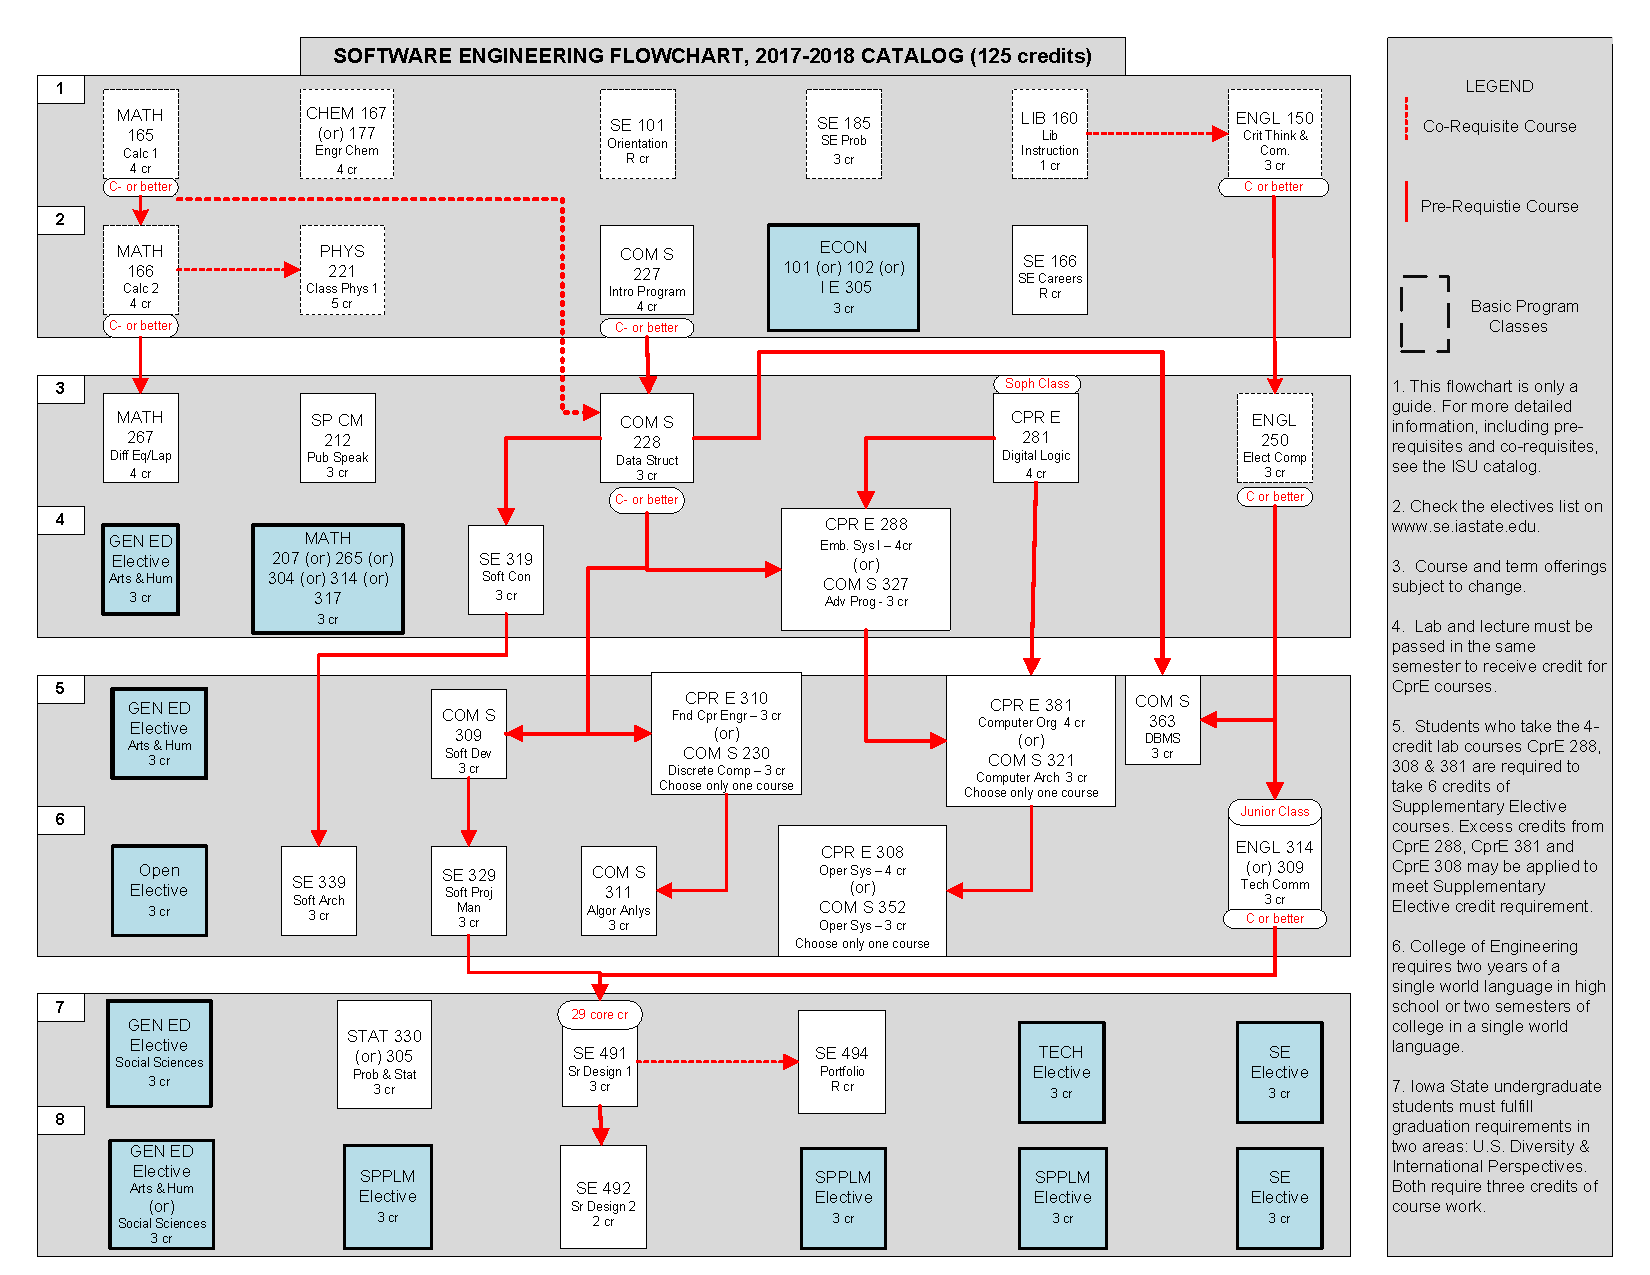
\includepdf[lastpage=1]{/home/collin/Documents/classwork/engl314/proposal/flowchart.pdf}

\end{document}
